\documentclass[tikz]{standalone}

\begin{document}

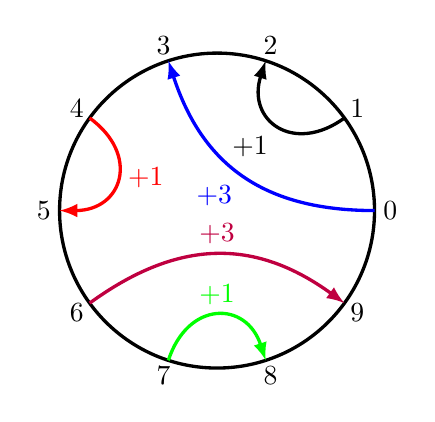
\begin{tikzpicture}[very thick, scale=2]
    \draw (0, 0) circle (1);
    \draw[black, -latex] ({360/10}:1) .. controls ({1*360/10}:.6) and ({2*360/10}:.6) .. ({2*360/10}:1) node[midway, below left]{+1};
    \draw[blue, -latex] ({0*360/10}:1) .. controls ({0*360/10}:.3) and ({3*360/10}:.3) .. ({3*360/10}:1) node[midway, below left]{+3};
    \draw[red, -latex] ({4*360/10}:1) .. controls ({4*360/10}:.6) and ({5*360/10}:.6) .. ({5*360/10}:1) node[midway, right]{+1};
    \draw[green, -latex] ({7*360/10}:1) .. controls ({7*360/10}:.6) and ({8*360/10}:.6) .. ({8*360/10}:1) node[midway, above]{+1};
    \draw[purple, -latex] ({6*360/10}:1) .. controls ({6*360/10}:.3) and ({9*360/10}:.3) .. ({9*360/10}:1) node[midway, above]{+3};
    \foreach \i in {0, ..., 9} {
        \draw ({\i*360/10}:1.1) node{\i};
    }
\end{tikzpicture}

\end{document}
